\documentclass{article}
\usepackage{amsmath, sfmath, multicol, tkz-euclide, array, enumerate, tcolorbox, tabularray}
\renewcommand{\familydefault}{\sfdefault}
\setlength{\parindent}{0cm}
\pagestyle{empty}
\usepackage[left=1in, top=0.5in, right=1in, bottom=0.5in]{geometry}
\tikzset{>=stealth}
\tcbset{colback=white}

\newcounter{example}[section]
\newenvironment{example}[1][]{\refstepcounter{example}\par\medskip
   {\color{red}\textbf{Example~\theexample. #1}}}{\medskip}

\begin{document}

\section*{Compositions of Isometries}

\begin{tcolorbox}[colframe=orange!70!white, coltitle=black, title=\textbf{Today I Can}]
\begin{enumerate}
    \item Perform successive transformations.
\end{enumerate}
\end{tcolorbox}
\bigskip

\begin{tcolorbox}[colframe=black!20!white, opacitybacktitle=0.1, coltitle=black, title=\textbf{Isometry}]
A transformation that preserves distance or length; \textit{i.e.} the pre-image and image are congruent.
\end{tcolorbox}
\bigskip 

The isometries we have studied so far are
\begin{itemize}
    \item Translations
    \item Reflections
    \item Rotations
\end{itemize}
\bigskip 

\begin{tcolorbox}[colframe=black!20!white, opacitybacktitle=0.1, coltitle=black, title=\textbf{Composition of Isometries}]
The result when one isometry is applied to after another.
\end{tcolorbox}
\bigskip 

\begin{example}
Translate $\triangle ABC$ 2 units right and 3 units down. Then reflect that result across the $x$-axis.
\newline

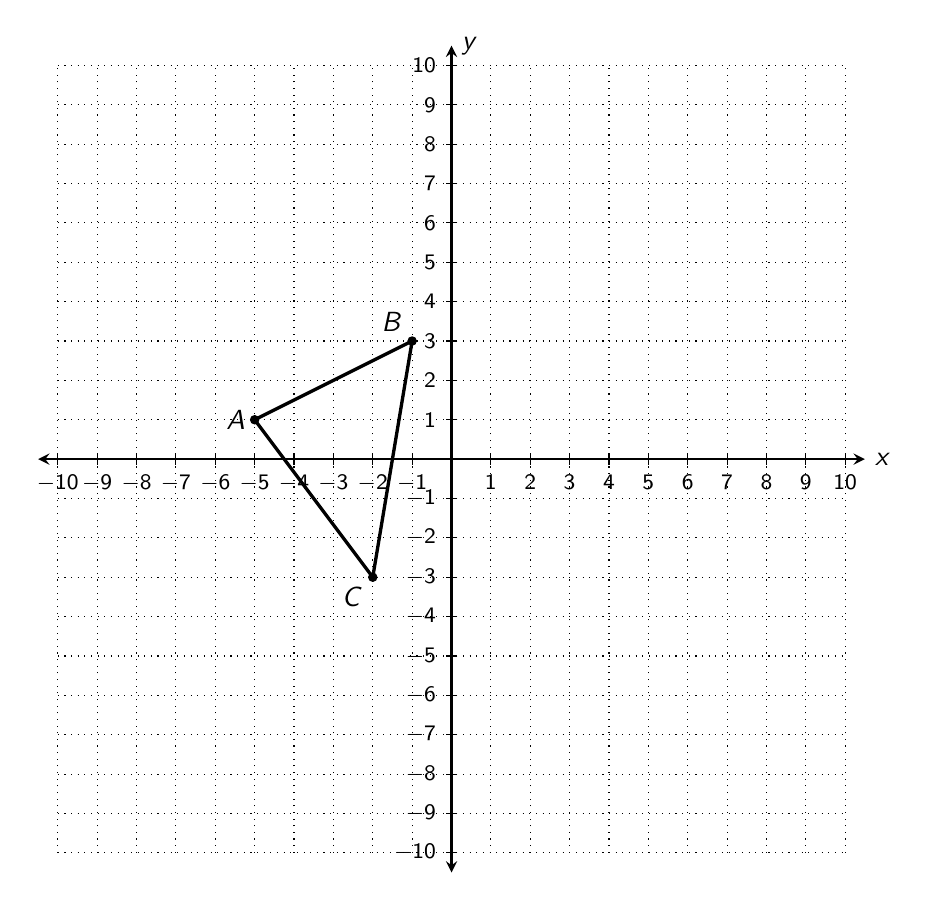
\begin{tikzpicture}[scale=0.5]
\draw[<->, thick] (-10.5,0) -- (10.5,0) node [right] {$x$};
\draw[<->, thick] (0,-10.5) -- (0,10.5) node [right] {$y$};
\draw[dotted] (-10,-10) grid (10,10);
\foreach \x in {-10,...,-1,,1,...,10}
\draw (\x, 0.15) -- (\x,-0.15) node [below] {\footnotesize $\x$};
\foreach \y in {-10,...,-1,,1,...,10}
\draw (0.15,\y) -- (-0.15,\y) node [left] {\footnotesize $\y$};
\coordinate (A) at (-5,1);
\coordinate (B) at (-1,3);
\coordinate (C) at (-2,-3);
\draw[fill=black] (-5,1) circle (3pt);
\draw[fill=black] (-1,3) circle (3pt);
\draw[fill=black] (-2,-3) circle (3pt);
\node at (A) [anchor = east] {$A$};
\node at (B) [anchor = south east] {$B$};
\node at (C) [anchor = north east] {$C$};
\draw [very thick] (A) -- (B) -- (C) -- cycle;
\end{tikzpicture}
\end{example}

\newpage 

\begin{example}
Rotate $\triangle ABC$ $90^\circ$ counterclockwise. Then reflect that result across the $y$-axis.
\newline

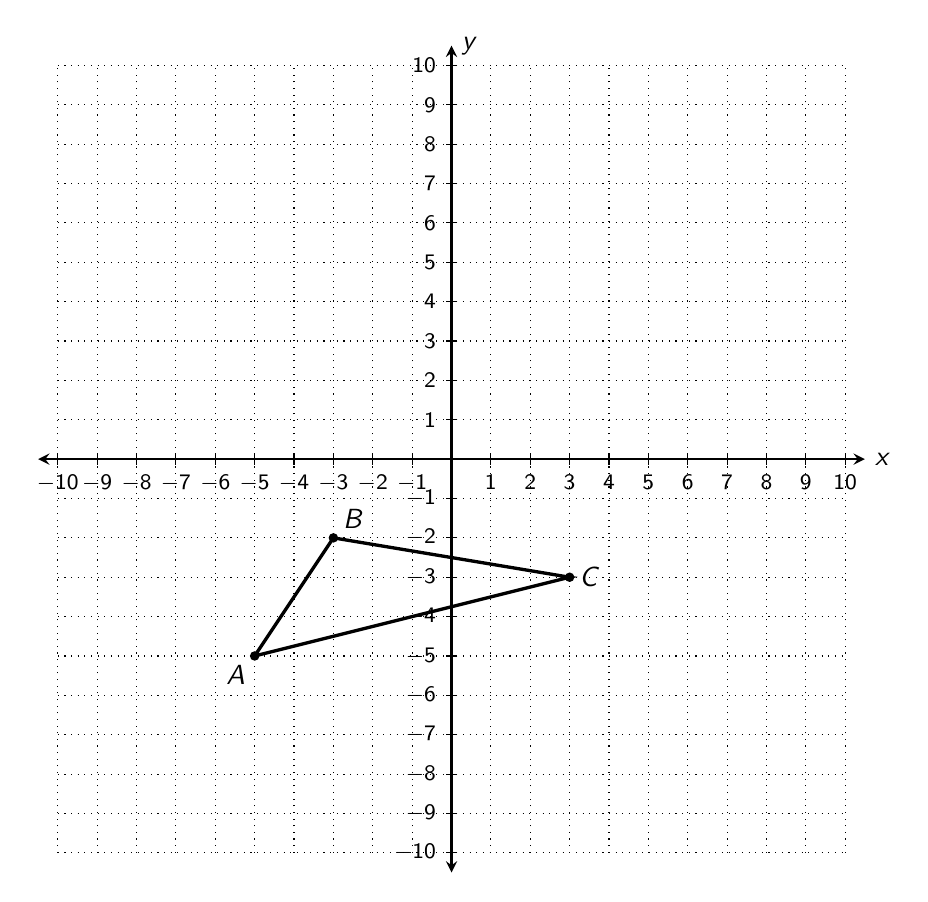
\begin{tikzpicture}[scale=0.5]
\draw[<->, thick] (-10.5,0) -- (10.5,0) node [right] {$x$};
\draw[<->, thick] (0,-10.5) -- (0,10.5) node [right] {$y$};
\draw[dotted] (-10,-10) grid (10,10);
\foreach \x in {-10,...,-1,,1,...,10}
\draw (\x, 0.15) -- (\x,-0.15) node [below] {\footnotesize $\x$};
\foreach \y in {-10,...,-1,,1,...,10}
\draw (0.15,\y) -- (-0.15,\y) node [left] {\footnotesize $\y$};
\coordinate (A) at (-5,-5);
\coordinate (B) at (-3,-2);
\coordinate (C) at (3,-3);
\draw[fill=black] (A) circle (3pt);
\draw[fill=black] (B) circle (3pt);
\draw[fill=black] (C) circle (3pt);
\node at (A) [anchor = north east] {$A$};
\node at (B) [anchor = south west] {$B$};
\node at (C) [anchor = west] {$C$};
\draw[very thick] (A) -- (B) -- (C) -- cycle;
\end{tikzpicture}
\end{example}

\vfill 

\begin{example}
Rotate $\triangle ABC$ $180^\circ$. Then reflect that result across the line $x=1$.
\newline

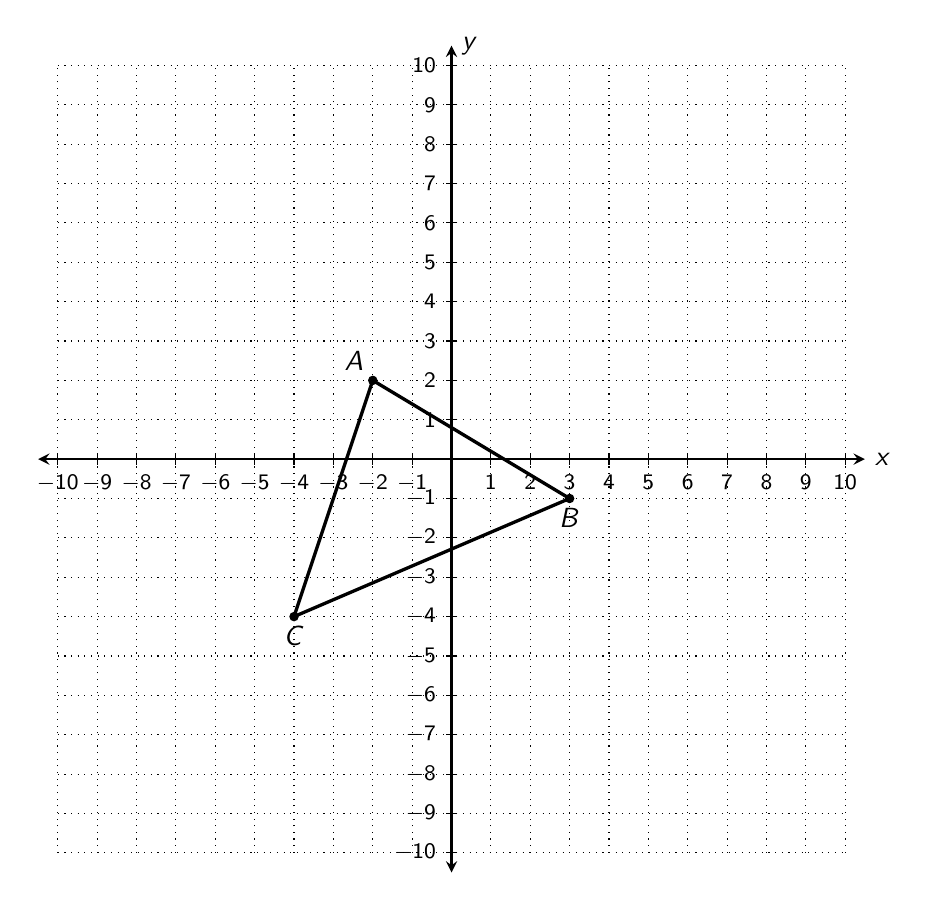
\begin{tikzpicture}[scale=0.5]
\draw[<->, thick] (-10.5,0) -- (10.5,0) node [right] {$x$};
\draw[<->, thick] (0,-10.5) -- (0,10.5) node [right] {$y$};
\draw[dotted] (-10,-10) grid (10,10);
\foreach \x in {-10,...,-1,,1,...,10}
\draw (\x, 0.15) -- (\x,-0.15) node [below] {\footnotesize $\x$};
\foreach \y in {-10,...,-1,,1,...,10}
\draw (0.15,\y) -- (-0.15,\y) node [left] {\footnotesize $\y$};
\coordinate (A) at (-2,2);
\coordinate (B) at (3,-1);
\coordinate (C) at (-4,-4);
\draw[fill=black] (A) circle (3pt);
\draw[fill=black] (B) circle (3pt);
\draw[fill=black] (C) circle (3pt);
\node at (A) [anchor = south east] {$A$};
\node at (B) [anchor = north] {$B$};
\node at (C) [anchor = north] {$C$};
\draw[very thick] (A) -- (B) -- (C) -- cycle;
\end{tikzpicture}
\end{example}

\vfill 

\end{document}
